\documentclass{article}
\usepackage[utf8]{inputenc}

\title{SciComp2017 HW1}
\author{Dmitriy Salnikov}
\date{October 2017}

\usepackage{natbib}
\usepackage{graphicx}
\usepackage{float}
\usepackage{hyperref}
\usepackage{amsfonts}


\hypersetup{
    colorlinks=true,
    urlcolor=red,
}

\begin{document}

\maketitle

\href{https://github.com/grapefroot/skoltech}{Please find the code HERE}

\section{Problem 1}
If $40\% $ of the program is not parallelizable, then by the application of Amdahl's law maximum achievable speedup is $\frac{100}{40} = 2.5$ 1/0.4 = 2.5. The efficiency of the two fold setup is $\frac{1}{2*(0.4 + 0.6/2)} = \frac{5}{7}$  

\section{Problem 2}
Each process uses their rank to gets the equal patch of files in the order that python's os.listdir() puts them in. Then we calculate the number of lines using the standard python tools and reduce it to the process with the rank 0. 


\section{Problem 3}

\href{http://www.spoj.com/status/DISUBSTR,grapefroot/}{link to SPOJ submission}

Consider the string $s$. Z function was used to solve the problem. If we consider the position i in the string, then Z function of i is the length of a maximum prefix of the string that is equal to the substring starting from i. Z function can be easily computed in O(length(s)). So, we can compute the number of different substrings of a string as follows: On each step we add symbols from the initial string one by one, starting from one symbol, and calculate the amount of new substrings, that are introduced by adding a new symbol. Consider we add a symbol $c$ to $s$ $s_new = s+c$. Let's count amount of new substrings that this symbol introduced. The claim is that this amount is exactly \[newStrings =  max(z function(reverse(s))) - length(s). \]. To show that this is true, consider reversed s and it's z function array. Then, we need to find all unique new prefixes introduced by the addition of the last element. The biggest prefix is corresponds to the max of the z function. All shorter prefixes also qualify. So,on each step we get exactly max(z) - length(s).
The running time is $O(length(s))^2$ since calculation of Z function array is $O(length(s))$ and this needs to be done $O(length(s))$ times.



\section{Problem 4}
At first I wanted to approach the problem as linear programming, but while searching for a scipy optimizer found more suitable option. This problem can be though of as the linear sum assignment minimization if you think of student rank vector as the costs for teaching the student this course. Then, it's clear that the same objective is minimized. 

Here's the objective function error, when number of experiments is 1000, matrix size is 30

\vspace{0.1in}

\begin{tabular}{| l | r |}
    \hline
   & mean error \\
  random & 434.001\\
  optimized & 23.001 \\
  \hline
\end{tabular}

\vspace{0.1in}

\begin{figure}[H]
    \centering
    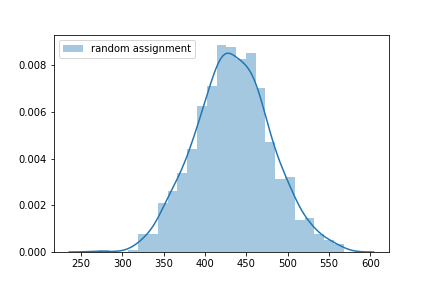
\includegraphics[scale=0.5]{random.png}
    \caption{random assignment distribution histogram}
    \label{fig:random}
\end{figure}

\begin{figure}[H]
    \centering
    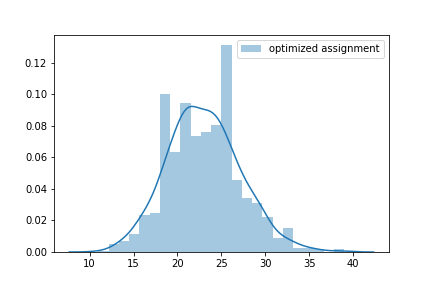
\includegraphics[scale=0.5]{optimized.png}
    \caption{optimized assignment distribution histogram}
    \label{fig:optimize}
\end{figure}

Big improvement is observed compared to the random assignment.


\section{Problem 5}

let $10^{-5} = x$

Consider N iid standard uniform random variables on the interval [0, 1]. Notice, that \[ P(r > x) = P(min_{1 \le n < m \le N}|x_n - x_m| \ge x) = N! * P(r \land X_{(1)} < X_{(2)} < X_{(3)} < \dots < X_{(N)}) \]

To estimate that we need to calculate the volume of the set of \[ V =  \{(x_1, \dots, x_N): \forall_{0 < i < n} \; (x_{i+1} - x_{i}) \ge x\} \]

Now, let's consider map \[f (x_1, \dots, x_N) \rightarrow (x_1, x_2 - x, x_3 - 2x, \dots, x_N - (N-1)x) \]. This map can be represented as a lower-triangular map with ones on the main diagonal. This, this map preserves the volume of the set.

The volume of f(V) is volume of \[ \{((x_1, \dots, x_n)) \in [0, 1 - (N-1)*x]^N: \forall_{i=2, \dots, N-1} \; y_i \le y_{i+1} \} \]

This seems to equal to $\frac{[0, 1 - (N-1)*x]^N}{n!}$

Then, \[ P(r > x) = (1-(N-1)x)^{N} = (1 - 999*10^{-5})^{1000} \approx 4.4*10^{-5} \] 

Thus, the probability of r being more than $10^{-5}$ is very low and in fact much higher than 10\% that was provided in the example.  

Concluding, our observation doesn't contradict the hypothesis of generating independent uniformly distributed random numbers.

\end{document}
